\chapter{Cosmology}\label{cosmology}
\pagecolor{gray}\afterpage{\nopagecolor}
\newpage
blah blah blah
\pagecolor{gray}\afterpage{\nopagecolor}
\fontfamily{pzc}
\selectfont

\newpage
\normalfont
\changepage{9cm}{9.4cm}{-4.7cm}{-4.7cm}{}{-4.5cm}{}{}{}
%\noindent\rule{\textwidth}{\textheight}
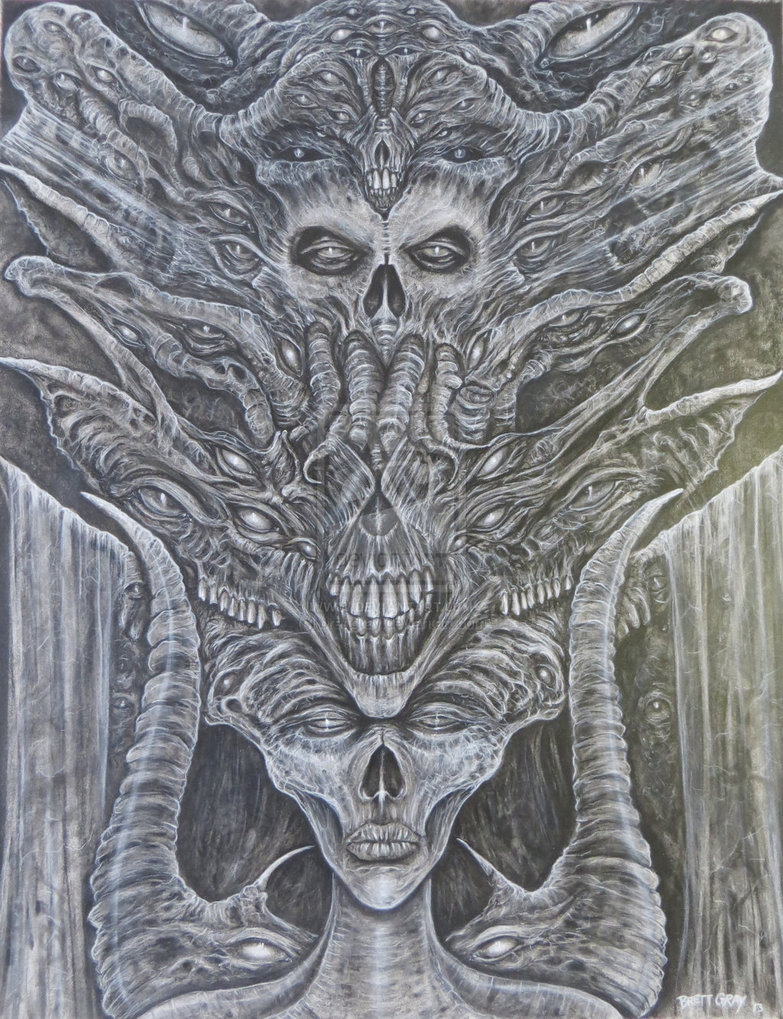
\includegraphics[width=\textwidth,height=\textheight]{priestess}
\newpage

%restoring the standard settings
\changepage{-9cm}{-9.4cm}{4.7cm}{4.7cm}{}{4.5cm}{}{}{}

\section{Creation Myths} In the beginning there was the void. Without warning came thought, unattached ambiguous thought. This thought soon grew and spawned the first light. From light came the memory of the dark and from that memory thought grew and created the world and the heavens. From the earth humans and animals grew. Men and animals had their own thoughts as well and this eventually spawned differences. These differences spawned women and different species. These differences created hatred and love, and from that strength and weakness, predator and the prey.

Communities formed to protect one from another and soon war. The conflict spawned more complex thoughts and questions. Soon the Gods were imagined and like all before, the Gods were different from one another. Gods ruled all the lesser beings and also warring with one another. These wars ravaged the world; civilizations grew from the conflict only to fall only to be replaced by newer and greater ones. The Gods depend on the conviction of their followers and as followers fall in these wars, Gods disappear, forgotten.

Humans became the dominate species and created technological wonders that replaced many Gods. The other species found comfort in lands humans would not claim. Some Gods who felt their time was at an end created Gates for them and their followers to retreat through. These Gates served as their ultimate refuge to the world, and lead them to a new world. As only three Gods remained, and would later be known as The Lords of Ends. Wars became more common. Communities were shattered; families butchered one another for little or no reason. Finally the greatest of all factions created a weapon that one ends all wars, all that ended was civilization.

With the world ravaged, the surviving creatures are left alone once again. None of survivors wished to remember the Lords of Ends and soon these Gods also died. One human dedicated himself to studying the lost arts and in time developed once forbidden arts. He mastered once forgotten arts of the old world and mastered all schools of magic. His students worshiped him and his power grew stronger and became the first human to truly ascend to that of godhood. He soon discovered the Gates and opened them. Some opened up violent worlds with even more violent and angry gods. Conflict began a new and the Gods returned to a new world and brought forth a new age.

%\begin{framed}\centering
% What you have here is a pantheon of recurring "pseudomythological" entities and a collection of arcane books that supposedly yield insights into the mythology.
% \end{framed}

\newpage
\section{Haeckel Pantheon}

\begin{tabular}{l | p {8 cm} | l}
    Deity & Domains & Worship Centers \\
    \hline
    \hline
    Aratron & Knowledge, Memory, Thought, Imagination, Magic, Arcane, Divine, Rune, Language, Wards & \\
    \hline
    Junon & Community, Family, Home, Judgement, Divine, Light, Stars, Knowledge, Moon & Midgaard \\
    \hline
    Alesia & Charm, Love, Lust, Family, Community, Law, Tyranny, Slavery, Revelry & \\
    \hline
    Gigas & Law, Loyalty, Nobility, Judgement, Leadership, Glory, Honour, Heroism, Strength, Resolve, Tactics & Ablon \\
    \hline
    The Priest King & Good, Redemption, Healing, Restoration, Resurrection, Judgement, Divine, Matyr, Purity, Protection, Community, Revelation & Midgaard\\
    \hline
    The Dyad & Charm, Love, Lust, Family, Cooperation, Loyalty & Brouliard \\
    \hline
    Ma'asei & Heroism, Glory, Honour, Inevitable, Explorer, Resolve & Ubris Furor \\
    \hline
    Magnus, Dante & & \\
    Secretum & & \\
    Nostra & & \\
    Mewgner & & \\
    The Hanged Man & & Nosquam \\
    Charon & & North Wall\\
    Sich & & \\
    Ra Herakht & & Abyssimiar \\
    Tinu & & \\
    Phex Eris & & Avalonia \\
    Waddell & & \\
    Neyord & & \\
    Asint & & \\
    Ignis & & \\
    Janus Thurinus & & South Midgaard \\
\end{tabular}


\begin{multicols}{2}
\subsection{Aratron} Master of the Divine, Lord of Aether, Master of all Mysteries, Divine Immanence.

Born a human and ascended to Godhood. Aratron is one of the survivors of the first world. He spent the last years as a mortal studying the lost arts of the old world and eventually developed the arts of Magic. His wisdom and power became so great that it propelled him to that of the Gods. He quickly grew lonely and curious as to the fate of the old Gods. This curiosity leads of to the Gates which the old Gods stepped through to avoid the coming disaster which ended the First World. He then opened all the Gates, returning all the exiled Gods and their followers to the New World.

Aratron is often associated with the God Nostra, whom travel through all seven Gates. Followers of both beliefs will often help one another and very rarely quarrel. Some of his followers argue with whether they should seek to be as Aratron and gain more power, or if such a task will anger the God and see such a task as a challenge.

The Church of Aratron tasks itself with preserving knowledge and perusing mystical arts. Certain sects aim to emulate their God and attempt to ascend to the heavens themselves, while others believe their God survived as a warning and that great power must be kept under control lest the world remakes itself yet again. The institution itself holds the later view, regulating magic users across Haeckel and even providing shelter to those who are hunted by mage slayers. A number of territories will respect such refuges out of fear of the Church's wraith. The Church however has never shown an act of aggression on non magic users. Many of these Churches can be found amongst universities, for they serve more as schools rather than places of worship.

Aratron is often depicted as wearing a white robe with a red cape. In his right hand is a wand raised towards the heaven, while his left hand is pointing to the earth. This gesture has multiple meanings, but is endemic to the Mysteries, symbolizing divine immanence, the ability of the magician to bridge the gap between heaven and earth. A table is often shown to be in front of Aratorn, on the table are the symbols that signify the classical elements of earth, air, fire and water. Beneath are roses and lilies changed into garden flowers, to show the culture of aspiration or symbolizing that he existed when the world was made anew.

Head masters of Aratron's flock will adorn a White robe covered by a red cape. The clothes that Aratron is often depicted wearing. Emissaries of Aratron are often highly coveted by those seeking great power.

Followers of Araton believe any book containing the knowledge of magic to be Holy Text. There are two books that are said to have been written by Aratron, one being The Gospel Vermillion and The Grammatica Aratron.

It is said that The Gospel Vermillion is was written with the blood of those who died from the First World and that it contained locations and designs of lost relics of power and that the pages have been scattered. The Grammatica Aratron is said to contain every spell that can ever be known and that these pages have also been scattered.

Although there is no religious holiday there is one day a year in which the Church of Aratron opens its doors to a new neophyte and announces a new Adept.

\subsection{Junon} The Holy Mother, Holy Mother Church

\subsection{Alesia} Queen of the Gods, Goddess of Beautiful things, Goddess of Abundance, Mother of A Thousand

\subsection{Gigas} Emperor of the Gods, The All Father, Caesar Dominus

\subsection{The Priest King} The mortal representative of the Gods

\subsection{The Dyad} The Lovers, The Holy Couple, The Inseparable Two

\subsection{Ma'asei}

\subsection{Magnus, Dante} 

\subsection{Secretum}

\subsection{Nostra}

\subsection{Mewgner}

\subsection{The Hanged Man}

\subsection{Charon}

\subsection{Sich}

\subsection{Sanat}

\subsection{Ra Herakht}

\subsection{Tinu}

\subsection{Phex Eris} 

\subsection{Waddell}

\subsection{Neyord}

\subsection{Asint}

\subsection{Ignis}

\subsection{Janus Thurinus}

\end{multicols}

\section{Abyssimiar Pantheon}

\newpage
\section{The Seven Major Cosmologies of Haeckel}
\begin{multicols}{2}

Within Haeckel there is no defined cosmology that is 100\% correct. Scholars from all around the Known World agree or disagree on the topic. The Magic systems themselves are known to contradict each other - with most Magi's spells following their own personal theories. 

\subsection{Ptolemaic Model} Universe orbits about a stationary Oerth. Planets move in circular epicycles, each having a center that moved in a larger circular orbit (called an eccentric or a deferent) around a center-point near the Earth. The use of equants added another level of complexity and allowed astronomers to predict the positions of the planets. The most successful universe model of all time, using the criterion of longevity. It is also known as the Great System, its theoretical foundations written by the Scholar Almagest. Classification: geocentric, abyssimiar. 
\subsection{Medieval Philosophy} A universe that is finite in time and has a beginning proposed by Philosopher Philoponus who argues against the ancient notion of an infinite universe. Since then further logical arguments supporting it have been developed by philosophers and theologians in Midgaard.

\subsection{Cartesian Vortex} A system of huge swirling whirlpools of aethereal or fine matter produces what we would call gravitational effects. His vacuum was not empty. All space was filled with matter that swirled around in large and small vortices. Classification: Static (evolving), steady state, infinite, renaissance.
\subsection{Memonaic Central Fire} At the center of the Universe is a central fire, around which Oerth, Sun, Moon and planets revolve uniformly. The Sun revolves around the central fire once a year, the stars are immobile. The earth in its motion maintains the same hidden face towards the central fire, hence it is never seen. This is the first known non-geocentric model of the Universe. This model was first proposed by the Firegiant Stargazer Memonaic. Classification: pythagorean, ancient.
\subsection{Cyclic Oscillation} One cycle of existence is around 3000 years and the life of one universe around a million years. This Universal cycle is preceded by an infinite number of universes and to be followed by another infinite number of universes. Includes an infinite number of universes at one given time. Central to this belief is the notion of the everlasting soul that reincarnates its self with each cycle; thus the pool of souls in reality never changes in number.
\subsection{Celestial Sphere} Spherical earth is surrounded by concentric celestial spheres. Universe exists unchanged throughout eternity. Contains a fifth element, called aether (later known as quintessence in Brouliard), added to the four Classical elements. This model is deemed heretical in Midgaard.

\subsection{Absolute Time and Space theorum} According to Magi Arakaban, absolute time exists independently of any perceiver and progresses at a consistent pace throughout the universe. Unlike relative time, Arakaban believed absolute time was imperceptible and could only be understood mathematically. According to Arakaban, humans are only capable of perceiving relative time, which is a measurement of perceivable objects in motion (like the moon or sun). From these movements, we infer the passage of time. These notions imply that absolute space and time do not depend upon physical events, but are a backdrop or stage setting within which physical phenomena occur.

\end{multicols}